% !TEX program = xelatex
% report.tex — 主文件
% 编译方式: xelatex (tectonic 或 XeLaTeX 均可)
\documentclass[12pt, a4paper]{article}

%% ===== 中文支持 =====
\usepackage{xeCJK}
\usepackage{fontspec}

% 字体路径（相对于编译目录，指向 assets/fonts/）
\setCJKmainfont[
  Path = ../assets/fonts/,
  BoldFont = NotoSerifCJKsc-Bold.otf
]{NotoSerifCJKsc-Regular.otf}
\setCJKsansfont[
  Path = ../assets/fonts/,
  BoldFont = NotoSansCJKsc-Bold.otf
]{NotoSansCJKsc-Regular.otf}
\setCJKmonofont[
  Path = ../assets/fonts/
]{NotoSansCJKsc-Regular.otf}

%% ===== 常用宏包 =====
\usepackage{geometry}
\geometry{left=2.5cm, right=2.5cm, top=2.8cm, bottom=2.8cm}

\usepackage{graphicx}
\usepackage{booktabs}
\usepackage{multirow}
\usepackage{amsmath, amssymb}
\usepackage{hyperref}
\hypersetup{
  colorlinks = true,
  linkcolor  = blue!60!black,
  citecolor  = green!50!black,
  urlcolor   = blue!70!black,
  pdfauthor  = {鲍明杨},
  pdftitle   = {从 3D Gaussian Splatting 到 Mesh：SuGaR 的快速复现、改动与实验分析}
}
\usepackage[numbers,sort&compress]{natbib}
\usepackage{enumitem}
\usepackage{xcolor}
\usepackage{listings}
\usepackage{caption}
\usepackage{subcaption}
\usepackage{float}
\usepackage[ruled,linesnumbered,vlined]{algorithm2e}
\SetAlgorithmName{算法}{算法}{算法列表}

%% ===== 自定义命令 =====
% \todo 标记待填内容
\newcommand{\todo}[1]{\textcolor{red}{\textbf{[TODO: #1]}}}
% 占位数字
\newcommand{\placeholder}[1]{\textcolor{red}{\textbf{（待填#1）}}}

%% ===== 代码高亮设置 =====
\lstset{
  basicstyle=\ttfamily\small,
  breaklines=true,
  frame=single,
  numbers=left,
  numberstyle=\tiny\color{gray},
  keywordstyle=\color{blue},
  commentstyle=\color{green!50!black},
  stringstyle=\color{red!60!black},
  showstringspaces=false
}

%% ===== 标题信息 =====
\title{\textbf{从 3D Gaussian Splatting 到 Mesh：\\SuGaR 的快速复现、改动与实验分析}}
\author{鲍明杨}
\date{2026 年 9 月 14 日}

%% ===== 正文 =====
\begin{document}
\maketitle

% ---- 摘要 ----
% abstract.tex — 摘要
\begin{abstract}
3D Gaussian Splatting（3DGS）以显式高斯基元为场景表示，实现了高质量实时渲染，
但其无组织的点云结构为表面网格（Mesh）提取带来了固有困难。
SuGaR（Surface-Aligned Gaussian Splatting）通过表面对齐正则化与 Poisson 重建
将高斯转化为三角网格，为渲染质量与几何可用性架起桥梁。

本报告在 truck 场景上从零复现了
3DGS（$\leq$\,7\,000 迭代）$\to$ Coarse SuGaR（$\leq$\,15\,000 迭代）
$\to$ Mesh 提取的基线流程，
并提出在 Poisson 重建前通过多视角深度一致性投票
剔除跨视角不自洽的虚假表面点。
通过基线与三组容差 $\tau\in\{0.05,\,0.02,\,0.01\}$ 的对照实验
（共 4 次完整提取）验证效果：
以 COLMAP 稀疏点云为参考，Chamfer 距离从 0.0531 降至 0.0390（$\tau{=}0.02$），
连通分量数从 4{,}851 降至 2{,}690；
代价是网格覆盖率从 92.9\% 降至 71.0\%。
渲染指标不受影响（Coarse PSNR 24.32\,dB、SSIM 0.848），
因改动仅作用于提取阶段。
本报告分析了改动的收益、代价与失败案例，并讨论了后续改进方向。
全部代码与复现命令已开源\footnote{\url{https://github.com/Find-Yit/temp_test}}。
\end{abstract}


% ---- 正文 ----
% sec1_method.tex — 第1节 方法
\section{方法}

% 本节介绍研究背景与所提改动方案。

\subsection{研究背景与问题}

3D Gaussian Splatting（3DGS）\cite{kerbl20233d} 以显式高斯基元为场景表示，
通过可微光栅化实现了高质量的实时渲染与快速训练。然而，原始 3DGS 产生的高斯集合
无组织、不具备拓扑结构，难以直接提取用于下游任务（物理仿真、编辑、3D 打印等）的
表面网格（Mesh）。
SuGaR（Surface-Aligned Gaussian Splatting）\cite{guedon2024sugar} 通过表面对齐
正则化策略，鼓励高斯基元贴合真实表面、协方差沿表面方向压缩，再借助 Poisson
表面重建从对齐后的高斯中提取三角网格。

本工作围绕三个核心问题展开：
\begin{enumerate}[label=(\arabic*)]
  \item 能否在有限预算（3DGS $\leq$ 7k 迭代，Coarse SuGaR $\leq$ 15k 迭代）下
        从零跑通完整的 3DGS $\to$ Coarse SuGaR $\to$ Mesh 提取流程？
  \item 能否提出一项进入训练或提取主流程的代码改动，并通过对照实验验证其效果？
  \item 改动是否带来了可观察的几何或渲染质量差异？若无，原因何在？
\end{enumerate}

\subsection{改动方案：Poisson 前的多视角深度一致性剔点}
\label{subsec:modification}

图~\ref{fig:pipeline} 给出了完整流程的全局视图，蓝色框为本文新增模块。

\begin{figure}[htbp]
  \centering
  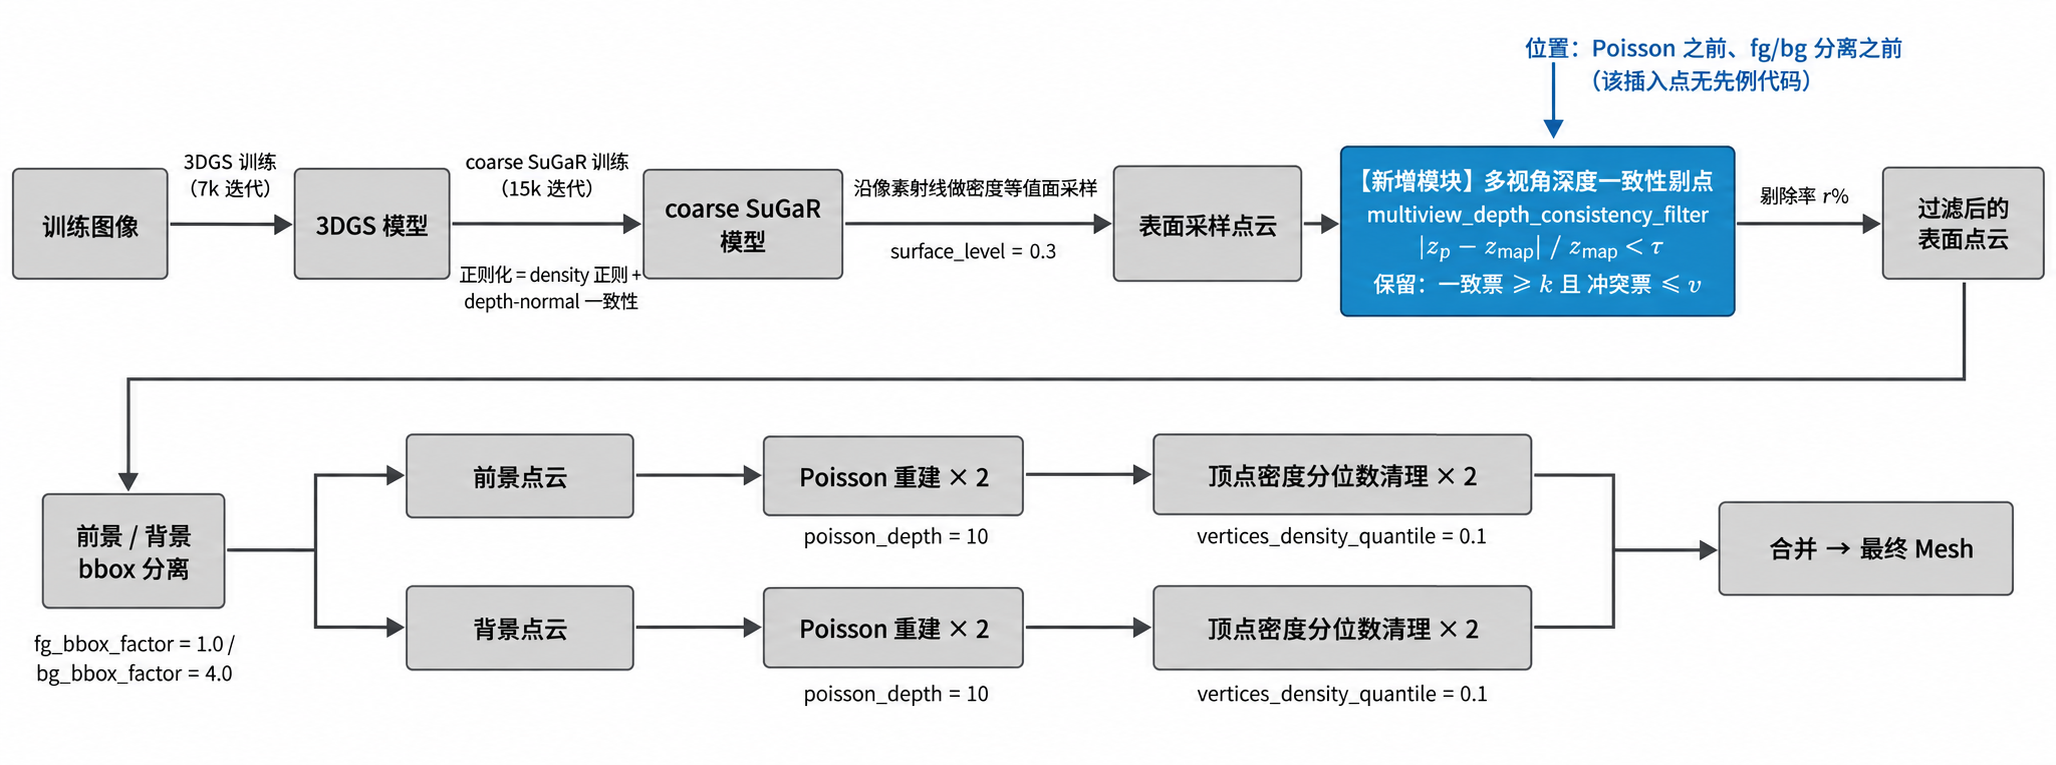
\includegraphics[width=\textwidth]{figures/改动示意图_A_流程.png}
  \caption{SuGaR Mesh 提取完整流程图。
  灰色节点为原始 SuGaR 流程，蓝色框为本文新增的多视角深度一致性剔点模块，
  插入位置为表面点采样之后、前景/背景分离与 Poisson 重建之前。}
  \label{fig:pipeline}
\end{figure}

%% ---------- 1.3.2 问题与动机 ----------
\subsubsection{问题与动机}
\label{sssec:motivation}

SuGaR \cite{guedon2024sugar} 的表面采样步骤在每个训练视角\emph{独立}进行：
沿该视角的射线找到密度等值面后即记录为表面点。
这种逐视角采样机制保证了每个点在其\emph{生成视角}下具有自洽的深度与法向，
但跨视角来看，某些采样点实际上悬浮在自由空间中——
它们对应的密度峰值只在单一视角的射线方向上存在，
并不被其他训练视角观测所支持。

这类\textbf{单视角自洽但跨视角不一致}的表面点主要产生两种伪影：
\begin{itemize}
  \item \textbf{漂浮几何}（floaters）：
        散布在场景空域中的孤立点簇，进入 Poisson 后形成
        膜状伪表面与薄壳连接；
  \item \textbf{背景壳}（background shells）：
        在远景区域（如天空、远处建筑面）由单色区域的密度累积产生的
        大面积伪表面，常表现为包裹整个场景的薄壳。
\end{itemize}

SuGaR 现有的两道后处理——统计离群点移除
与 Poisson 顶点密度分位数裁剪——
均基于局部几何统计，无法有效识别上述在几何分布上并不异常、
但在多视角一致性上不成立的虚假表面点。
图~\ref{fig:before-after} 以示意方式展示了剔点前后表面点云与 Poisson Mesh 的对比。

\begin{figure}[htbp]
  \centering
  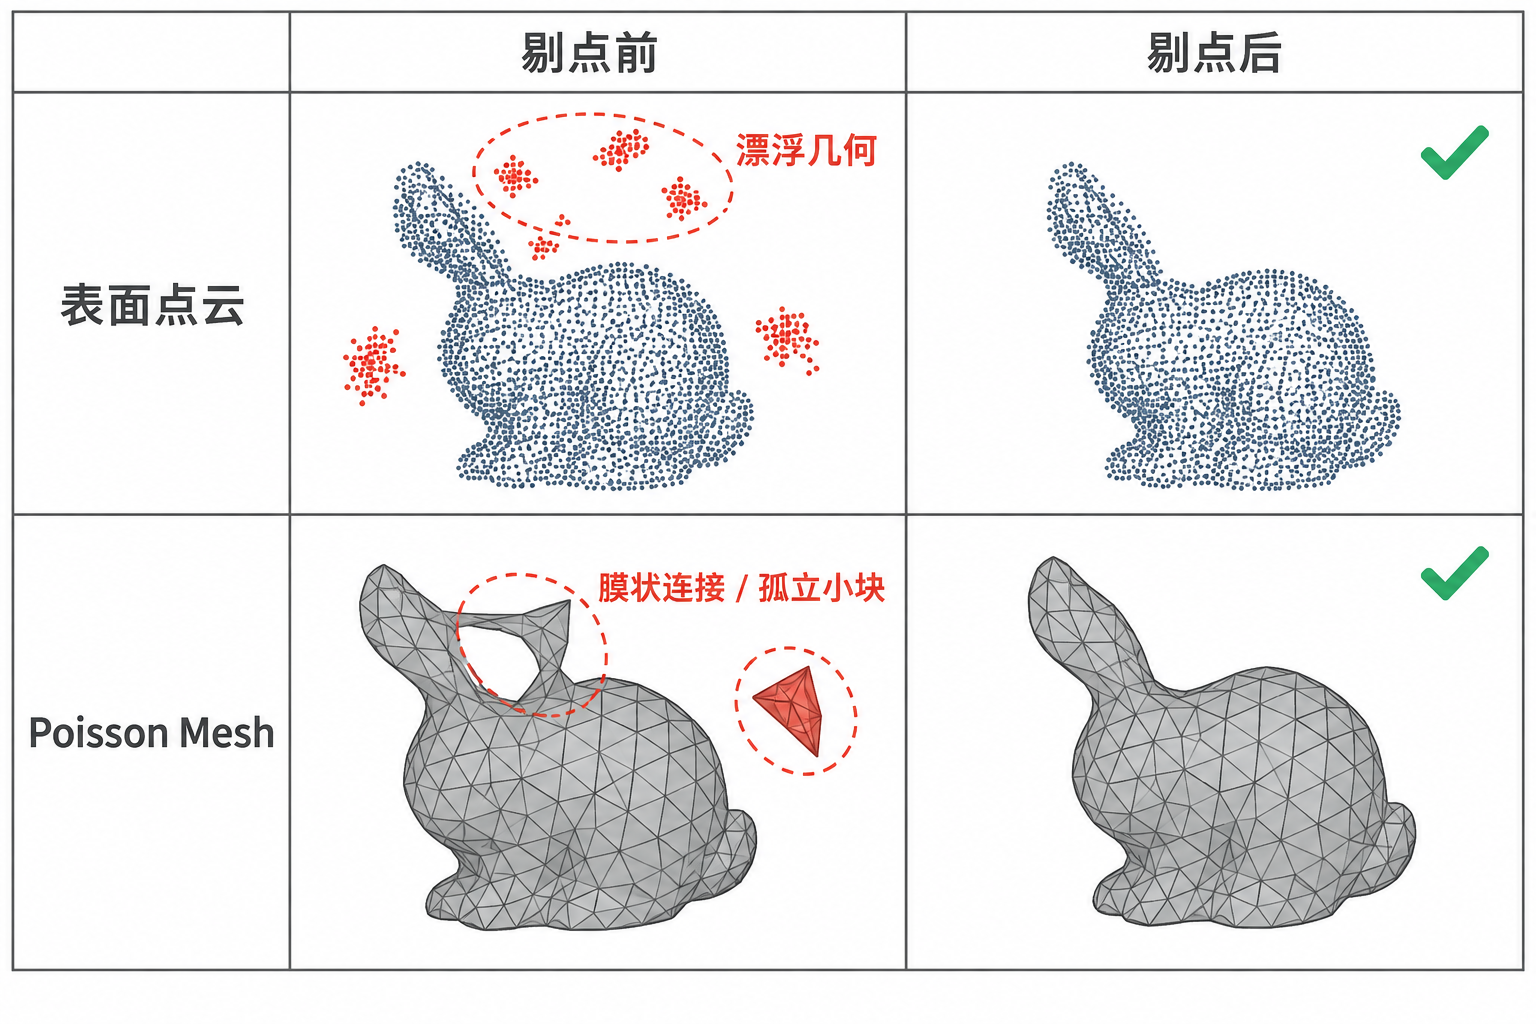
\includegraphics[width=0.85\textwidth]{figures/改动示意图_C_前后对比.png}
  \caption{剔点前后对比示意。
  上排：表面点云，剔点前含明显漂浮几何（红色标注），剔点后更干净。
  下排：Poisson Mesh，剔点前存在膜状连接与孤立小块，剔点后网格更紧凑。}
  \label{fig:before-after}
\end{figure}

%% ---------- 1.3.3 方法描述 ----------
\subsubsection{方法描述}
\label{sssec:method-detail}

\paragraph{符号定义。}
设 Coarse SuGaR 训练完成后，对某一 \texttt{surface\_level}
值采样得到的表面点集合为 $\mathcal{P} = \{p_i\}_{i=1}^{N}$，
训练相机集合为 $\mathcal{C} = \{c_j\}_{j=1}^{|\mathcal{C}|}$。
从 $\mathcal{C}$ 中均匀抽取 $M$ 个相机（固定 \texttt{seed}=0）
组成参考相机子集 $\mathcal{C}_M$。
对 $\mathcal{C}_M$ 中的每个相机 $c_j$，
预先用 SuGaR 的 \texttt{render\_depth\_and\_normal} 缓存其渲染深度图
$D_j \in \mathbb{R}^{H \times W}$。

\paragraph{判据。}
对点 $p_i$，将其投影到相机 $c_j$ 得到像素坐标 $(u, v)$ 与相机空间深度 $z_p$。
取深度图对应像素值 $z_{\mathrm{map}} = D_j(u, v)$。
定义以下三种投票：

\begin{itemize}
  \item \textbf{一致票}（consistent vote）：
        $|z_p - z_{\mathrm{map}}| < \tau \cdot z_{\mathrm{map}}$，
        即相对深度差在容差 $\tau$ 以内；
  \item \textbf{空域冲突票}（free-space conflict vote）：
        $z_p < z_{\mathrm{map}} - \tau \cdot z_{\mathrm{map}}$，
        即点明显浮在该视角已知表面\textbf{之前}的自由空间中；
  \item \textbf{无效}（不计票）：
        点落在相机 $c_j$ 视锥之外，或深度图对应像素无有效深度值。
\end{itemize}

\paragraph{保留条件。}
点 $p_i$ 被保留当且仅当同时满足：
\begin{equation}
  \label{eq:keep-condition}
  \underbrace{\sum_{j \in \mathcal{C}_M} \mathbf{1}[\text{一致}(p_i, c_j)]}_{\text{一致票数}} \;\geq\; k_{\min}
  \quad \text{且} \quad
  \underbrace{\sum_{j \in \mathcal{C}_M} \mathbf{1}[\text{冲突}(p_i, c_j)]}_{\text{冲突票数}} \;\leq\; v_{\max}
\end{equation}
其中 $k_{\min}$ 默认为2，
$v_{\max}$ 默认为1。
图~\ref{fig:vote-criterion} 以两个典型案例直观展示了投票判据的工作方式。

\begin{figure}[htbp]
  \centering
  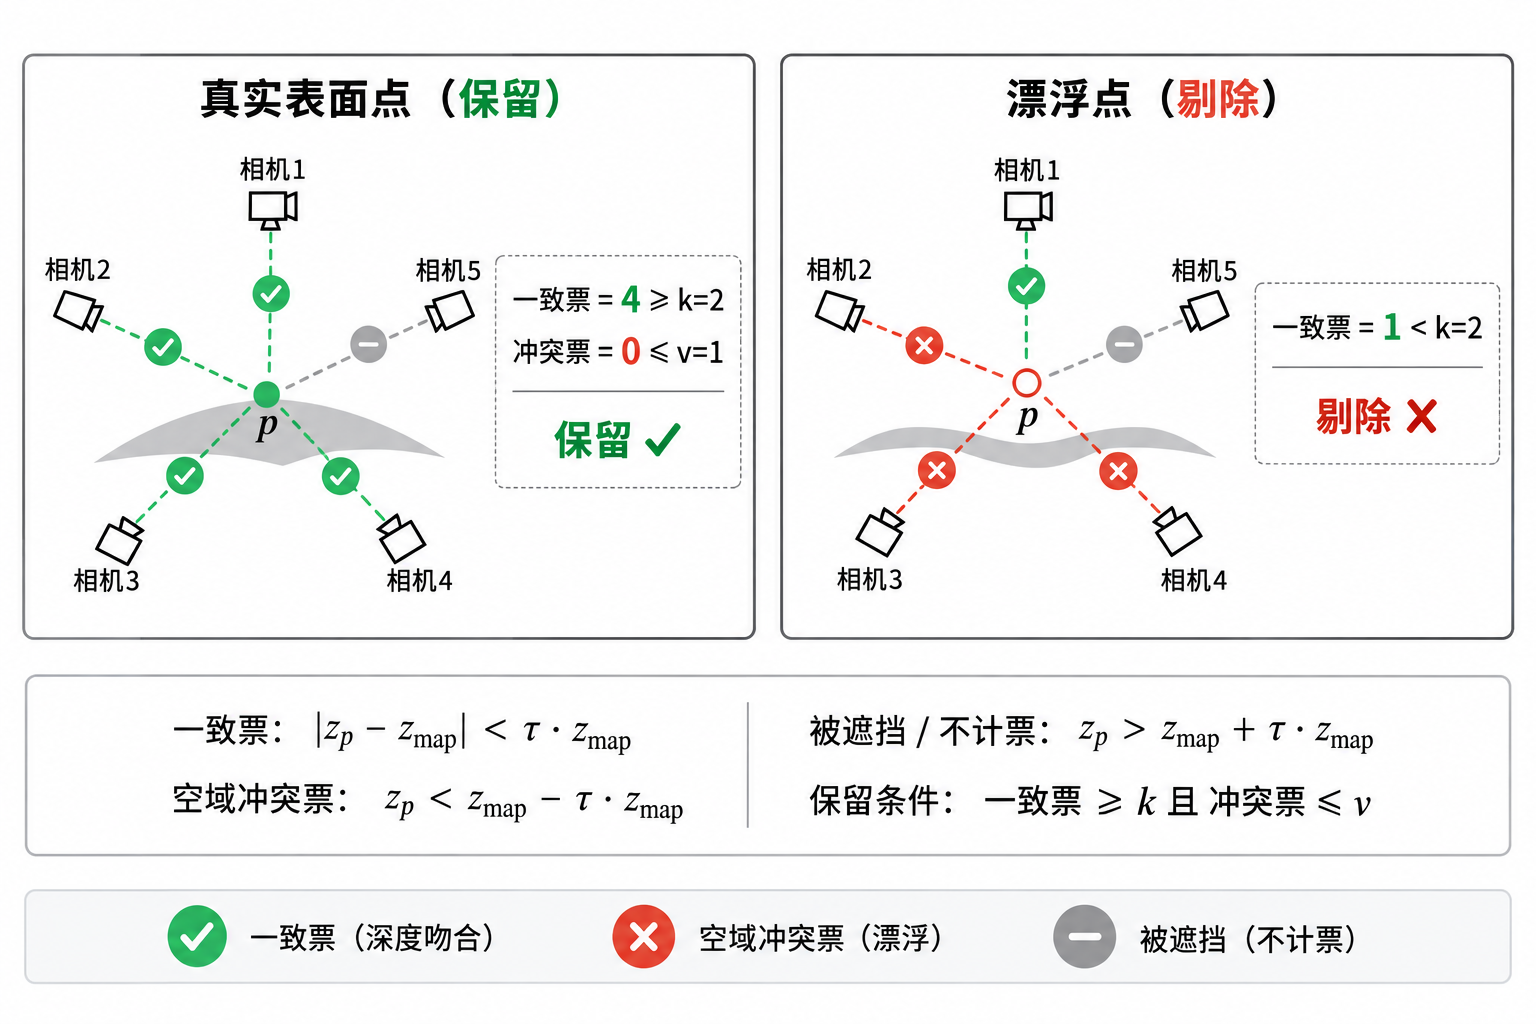
\includegraphics[width=0.9\textwidth]{figures/改动示意图_B_判据.png}
  \caption{多视角深度一致性投票判据示意。
  左：真实表面点获得 4 个一致票，满足保留条件（一致票 $\geq k{=}2$ 且冲突票 $\leq v{=}1$）。
  右：漂浮点仅获 1 个一致票且有 3 个冲突票，被剔除。
  绿色为一致票（深度吻合），红色为空域冲突票（漂浮），灰色为被遮挡（不计票）。}
  \label{fig:vote-criterion}
\end{figure}

全部超参数及默认值见附录表~\ref{tab:mv-hyperparams}，
其中 $\tau$ 为主要消融变量，扫描范围 $\{0.01, 0.02, 0.05\}$。
完整算法伪代码见附录算法~\ref{alg:mv-filter}。


% sec2_dataset.tex — 第2节 数据集与评测协议
\section{数据集与评测协议}

\subsection{数据来源与划分}

本实验使用 3DGS~\cite{kerbl20233d} 官方发布的 Tanks \& Temples 数据包中的
\textbf{truck} 场景。该数据集由 COLMAP~\cite{schoenberger2016sfm}
完成结构化运动恢复（Structure from Motion, SfM）与稀疏三维重建，
提供已标定内外参的多视角图像及稀疏三维点云。
训练与测试视角按 3DGS 标准划分 \texttt{llffhold=8}：
每隔~8 张取~1 张作为测试视角，其余为训练视角。
表~\ref{tab:data} 汇总了数据集概况。

\begin{table}[H]
\centering
\caption{数据集概况}
\label{tab:data}
\begin{tabular}{lcccc}
\toprule
\textbf{场景} & \textbf{图像总数} & \textbf{训练视角} & \textbf{测试视角} & \textbf{COLMAP 稀疏点数} \\
\midrule
truck & 251 & 219 & 32 & 136{,}029 \\
\bottomrule
\end{tabular}
\end{table}

\subsection{训练预算与提取参数}

基线流程各阶段的预算设置如下：
\begin{itemize}[nosep]
  \item \textbf{3DGS 预训练}：7{,}000 迭代，随机种子~0；
  \item \textbf{Coarse SuGaR 训练}：\texttt{num\_iterations}=15{,}000
        （迭代计数器从~7{,}000 起，实际优化约~8{,}000 步），
        采用密度估计 + 深度--法向一致性（dn\_consistency）正则；
  \item \textbf{Mesh 提取}：\texttt{surface\_level}=0.3，
        Screened Poisson~\cite{kazhdan2006poisson} 八叉树深度~10，
        顶点密度分位数裁剪阈值~0.1，抽简目标顶点数~1{,}000{,}000。
\end{itemize}

\subsection{评测协议}

几何评测采用\textbf{双参考}比较方案：
参考~A 为 3DGS 训练后的高斯中心点云（bbox 裁剪后~284{,}309 点），
参考~B 为 COLMAP 稀疏点云（bbox 裁剪后~56{,}988 点）。
裁剪区域由训练相机中心的轴对齐包围盒定义
（对角线长约~13.34 场景坐标单位）。
从网格表面均匀采样~1{,}000{,}000 个点，
随机种子固定为~0，
计算精度（Accuracy）、完整度（Completeness）、Chamfer 距离与
F-score（阈值取场景尺度对角线的~0.5\%、1\%、2\%）。
渲染指标（PSNR、SSIM、LPIPS）在全部~32 个测试视角上计算并取均值。

% sec3_results.tex — 第3节 结果
\section{结果}

\subsection{实验设置}

为验证第~\ref{subsec:modification}~节所述改动的有效性，设计了以下实验组别：

\begin{table}[H]
\centering
\caption{实验组别设置}
\label{tab:exp-groups}
\begin{tabular}{llll}
\toprule
\textbf{组别}     & \textbf{标识}    & \textbf{核心差异}              & \textbf{说明} \\
\midrule
基线               & Baseline         & 原始 SuGaR 提取流程            & 无剔点 \\
改动（$\tau{=}0.05$）  & Modified-0.05  & 多视角剔点\,$\tau{=}0.05$  & 剔除 25.5\% \\
改动（$\tau{=}0.02$）  & Modified-0.02  & 多视角剔点\,$\tau{=}0.02$  & 默认值，剔除 44.9\% \\
改动（$\tau{=}0.01$）  & Modified-0.01  & 多视角剔点\,$\tau{=}0.01$  & 剔除 59.2\% \\
\bottomrule
\end{tabular}
\end{table}

所有组别共享同一 3DGS 预训练检查点（7{,}000 迭代、\texttt{seed}=0）、
相同的 Coarse SuGaR 权重（\texttt{num\_iterations}=15{,}000）以及相同的
测试视角划分（\texttt{llffhold}=8，32 个测试视角）。
改动仅作用于 Mesh 提取阶段，不影响 3DGS 与 Coarse SuGaR 的训练过程。

\textbf{评价指标}包括五个维度：
\begin{itemize}[nosep]
  \item 渲染质量：测试视角 PSNR / SSIM / LPIPS（\S\ref{ssec:baseline-render}）；
  \item 几何精度：双参考 Accuracy / Completeness / Chamfer / F-score（\S\ref{ssec:baseline-geo}）；
  \item 拓扑质量：连通分量数、水密性、孔洞数等（\S\ref{ssec:baseline-topo}）；
  \item 覆盖度：网格渲染覆盖率与前景漏洞率（\S\ref{ssec:baseline-topo}）；
  \item 效率：各阶段墙钟时间、峰值显存与文件体积（\S\ref{ssec:baseline-topo}）。
\end{itemize}

% =====================================================================
\subsection{定量结果}
\label{ssec:baseline-results}

以下报告全部实验组别在 truck 场景上的定量结果。

% ---------- 渲染指标 ----------
\subsubsection{渲染指标}
\label{ssec:baseline-render}

表~\ref{tab:render-metrics} 给出 3DGS（7k 迭代）与 Coarse SuGaR 在 32 个测试视角
上的渲染质量。由于改动仅影响 Mesh 提取阶段，不改变 3DGS 或 Coarse SuGaR
的训练权重，因此所有组别共享同一 Coarse 模型，渲染指标恒等。

\begin{table}[H]
\centering
\caption{渲染指标（truck，32 测试视角均值）。
各组别共享同一 Coarse SuGaR 模型，故渲染指标与基线恒等。}
\label{tab:render-metrics}
\begin{tabular}{lccc}
\toprule
\textbf{模型} & \textbf{PSNR (dB) $\uparrow$}
               & \textbf{SSIM $\uparrow$}
               & \textbf{LPIPS $\downarrow$} \\
\midrule
3DGS（7k 迭代）   & 23.92 & 0.849 & 0.202 \\
Coarse SuGaR       & 24.32 & 0.848 & 0.217 \\
\bottomrule
\end{tabular}
\end{table}

% ---------- 几何指标 ----------
\subsubsection{几何指标}
\label{ssec:baseline-geo}

表~\ref{tab:geo-refA} 与表~\ref{tab:geo-refB} 分别给出以 3DGS 高斯中心（参考 A）
和 COLMAP 稀疏点云（参考 B）为基准的几何评测结果。
所有距离均以场景坐标为单位（场景对角线~$\approx$\,13.34）。
$\tau$ 越小，剔点越激进，几何精度（Chamfer / Completeness / F-score）一致改善，
但精度尾部（Accuracy P90）逐渐变差，反映了真实表面被误剔的趋势。

\begin{table}[H]
\centering\small
\caption{几何指标——参考 A（3DGS 高斯中心，284{,}309 点）}
\label{tab:geo-refA}
\begin{tabular}{@{}lcccc@{}}
\toprule
\textbf{指标} & \textbf{基线} & $\tau{=}0.05$ & $\tau{=}0.02$ & $\tau{=}0.01$ \\
\midrule
Chamfer L1 $\downarrow$          & 0.0326 & 0.0287 & 0.0242 & 0.0230 \\
\addlinespace
Accuracy 均值 $\downarrow$       & 0.0156 & 0.0184 & 0.0198 & 0.0220 \\
Accuracy 中位 $\downarrow$       & 0.0098 & 0.0103 & 0.0105 & 0.0110 \\
Accuracy P90 $\downarrow$        & 0.0291 & 0.0327 & 0.0343 & 0.0366 \\
\addlinespace
Completeness 均值 $\downarrow$   & 0.0495 & 0.0389 & 0.0286 & 0.0241 \\
Completeness 中位 $\downarrow$   & 0.0233 & 0.0183 & 0.0148 & 0.0138 \\
Completeness P90 $\downarrow$    & 0.1317 & 0.0995 & 0.0593 & 0.0490 \\
\addlinespace
F@0.5\% $\uparrow$              & 0.864 & 0.902 & 0.940 & 0.952 \\
F@1\% $\uparrow$                & 0.946 & 0.961 & 0.976 & 0.982 \\
F@2\% $\uparrow$                & 0.990 & 0.993 & 0.994 & 0.995 \\
\bottomrule
\end{tabular}
\end{table}

\begin{table}[H]
\centering\small
\caption{几何指标——参考 B（COLMAP 稀疏点，56{,}988 点）}
\label{tab:geo-refB}
\begin{tabular}{@{}lcccc@{}}
\toprule
\textbf{指标} & \textbf{基线} & $\tau{=}0.05$ & $\tau{=}0.02$ & $\tau{=}0.01$ \\
\midrule
Chamfer L1 $\downarrow$          & 0.0531 & 0.0455 & 0.0390 & 0.0361 \\
\addlinespace
Accuracy 均值 $\downarrow$       & 0.0242 & 0.0262 & 0.0279 & 0.0303 \\
Accuracy 中位 $\downarrow$       & 0.0033 & 0.0035 & 0.0036 & 0.0037 \\
Accuracy P90 $\downarrow$        & 0.0200 & 0.0239 & 0.0258 & 0.0287 \\
\addlinespace
Completeness 均值 $\downarrow$   & 0.0819 & 0.0648 & 0.0500 & 0.0419 \\
Completeness 中位 $\downarrow$   & 0.0480 & 0.0387 & 0.0307 & 0.0271 \\
Completeness P90 $\downarrow$    & 0.2005 & 0.1530 & 0.1044 & 0.0853 \\
\addlinespace
F@0.5\% $\uparrow$              & 0.751 & 0.807 & 0.862 & 0.885 \\
F@1\% $\uparrow$                & 0.888 & 0.920 & 0.949 & 0.963 \\
F@2\% $\uparrow$                & 0.963 & 0.973 & 0.979 & 0.982 \\
\bottomrule
\end{tabular}
\end{table}

% ---------- 拓扑 / 覆盖 / 效率 ----------
\subsubsection{拓扑、覆盖与效率}
\label{ssec:baseline-topo}

表~\ref{tab:topo-cov-eff} 汇总了网格拓扑质量、渲染覆盖度与效率指标。

\begin{table}[H]
\centering\footnotesize
\caption{拓扑、覆盖与效率指标（truck 场景）}
\label{tab:topo-cov-eff}
\begin{tabular}{llcccc}
\toprule
\textbf{类别} & \textbf{指标}
  & \textbf{基线} & $\tau{=}0.05$ & $\tau{=}0.02$ & $\tau{=}0.01$ \\
\midrule
\multirow{7}{*}{拓扑}
  & 顶点数 $V$           & 746{,}704
                                      & 665{,}745 & 574{,}239 & 455{,}839 \\
  & 面数 $F$             & 1{,}437{,}272
                                      & 1{,}295{,}321 & 1{,}121{,}525 & 890{,}054 \\
  & 连通分量数           & 4{,}851   & 3{,}279   & 2{,}690   & 2{,}261 \\
  & 最大分量面数占比     & 49.5\%    & 58.1\%    & 48.8\%    & 47.3\% \\
  & 边界边数             & 96{,}544  & 68{,}205  & 54{,}647  & 44{,}848 \\
  & 孔洞数（边界环）     & 7{,}970   & 6{,}206   & 5{,}480   & 4{,}598 \\
  & 水密                 & 否         & 否         & 否         & 否 \\
\midrule
\multirow{2}{*}{覆盖}
  & 网格覆盖率 $\uparrow$    & 92.9\% & 81.5\% & 71.0\% & 63.3\% \\
  & 前景漏洞率 $\downarrow$  & 6.7\%  & 18.0\% & 28.6\% & 36.3\% \\
\midrule
\multirow{6}{*}{效率}
  & 3DGS 训练            & 1.98\,min
                                      & \multicolumn{3}{c}{（共享）} \\
  & Coarse SuGaR 训练    & 15.84\,min
                                      & \multicolumn{3}{c}{（共享）} \\
  & Mesh 提取            & 5.98\,min & 4.79\,min & 4.30\,min & 3.91\,min \\
  & \textbf{总墙钟}      & \textbf{23.81\,min}
                                      & \textbf{22.62\,min}
                                      & \textbf{22.13\,min}
                                      & \textbf{21.74\,min} \\
  & 峰值显存（进程组）   & 10{,}098\,MiB
                                      & 8{,}274\,MiB & 8{,}274\,MiB & 8{,}274\,MiB \\
  & 网格文件体积         & 54.34\,MiB
                                      & 48.56\,MiB & 41.94\,MiB & 33.29\,MiB \\
\bottomrule
\end{tabular}
\begin{flushleft}
\footnotesize
"（共享）"表示该阶段在基线与改动之间相同（改动仅作用于提取阶段）。
\end{flushleft}
\end{table}

% ---------- 可视化 ----------
\subsubsection{可视化}
\label{ssec:baseline-vis}

图~\ref{fig:baseline-vis} 展示了基线提取网格的四个可视化视角。

\begin{figure}[htbp]
  \centering
  \begin{subfigure}[b]{0.48\textwidth}
    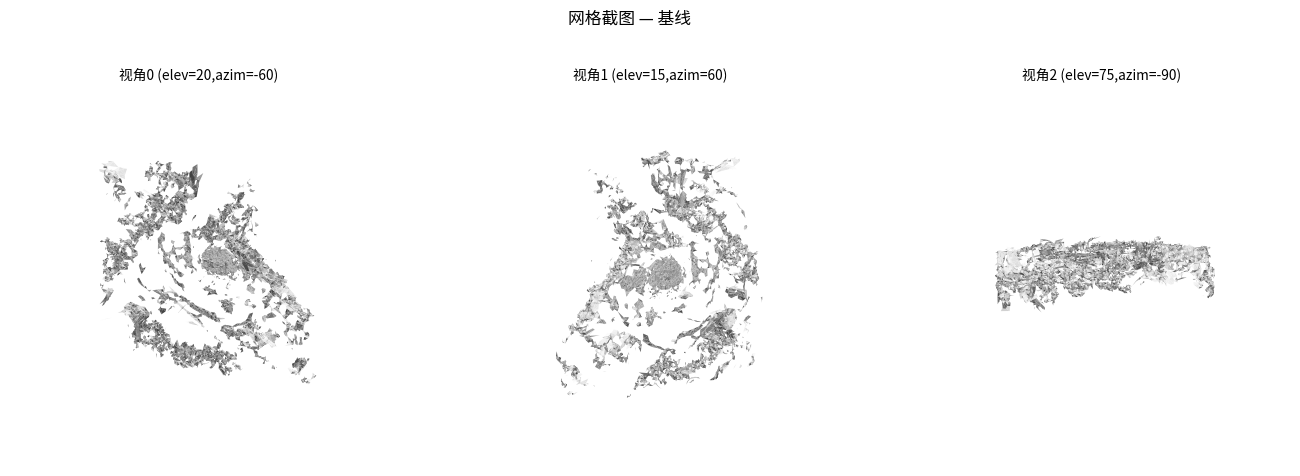
\includegraphics[width=\textwidth]{figures/网格截图_基线.png}
    \caption{提取网格整体视图}
    \label{fig:baseline-mesh}
  \end{subfigure}
  \hfill
  \begin{subfigure}[b]{0.48\textwidth}
    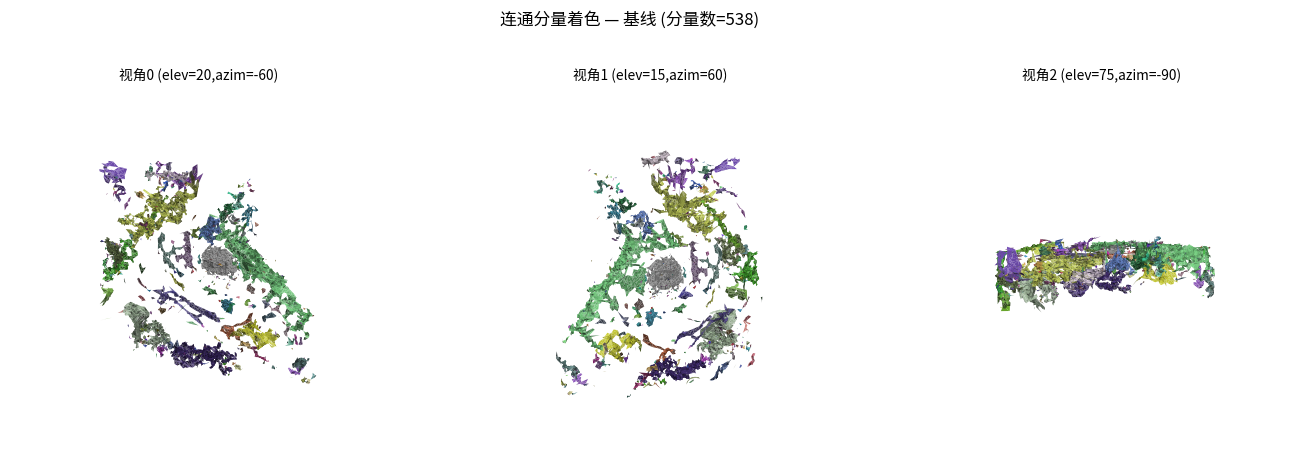
\includegraphics[width=\textwidth]{figures/连通分量着色_基线.png}
    \caption{连通分量着色（不同颜色代表不同分量）}
    \label{fig:baseline-components}
  \end{subfigure}

  \vspace{0.5em}

  \begin{subfigure}[b]{0.48\textwidth}
    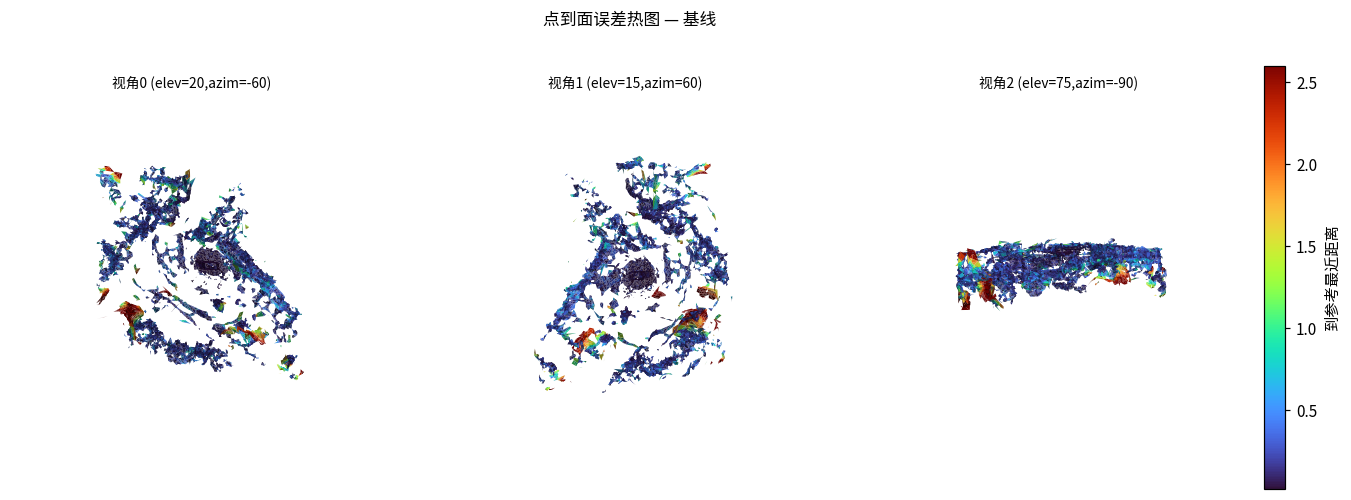
\includegraphics[width=\textwidth]{figures/误差热图_基线.png}
    \caption{几何误差热图}
    \label{fig:baseline-error}
  \end{subfigure}
  \hfill
  \begin{subfigure}[b]{0.48\textwidth}
    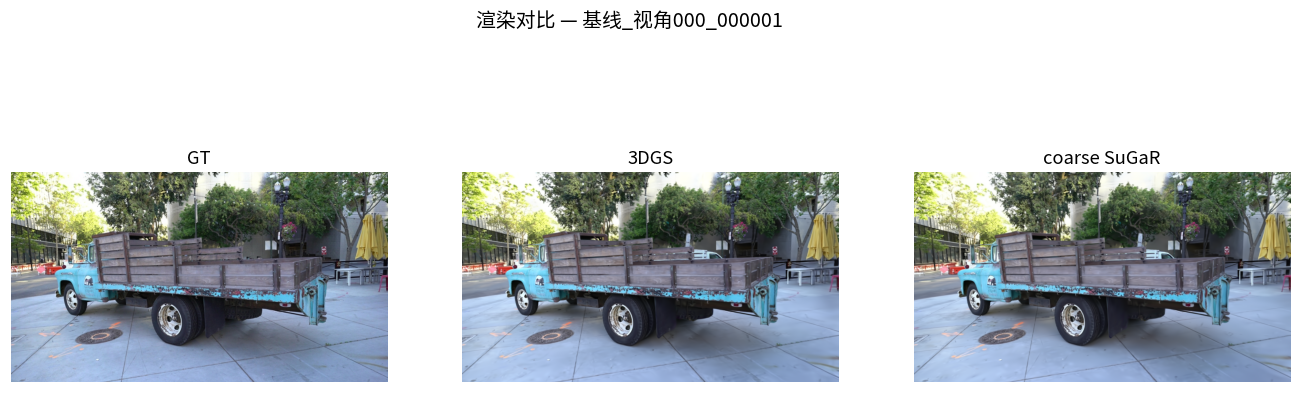
\includegraphics[width=\textwidth]{figures/渲染对比_基线_视角000_000001.png}
    \caption{测试视角渲染效果（视角~0）}
    \label{fig:baseline-render}
  \end{subfigure}
  \caption{基线 SuGaR Mesh 提取可视化（truck 场景）。
  (a) 整体网格；
  (b) 4{,}851 个连通分量以颜色区分，可见大量小碎片散布于主体之外；
  (c) 到参考点云的距离误差热图；
  (d) 从测试视角的渲染结果与真值对比。}
  \label{fig:baseline-vis}
\end{figure}

图~\ref{fig:heatmap-comparison} 以统一色标展示了基线与改动（$\tau{=}0.02$）
的几何误差热图对比。

\begin{figure}[htbp]
  \centering
  \begin{subfigure}[b]{0.48\textwidth}
    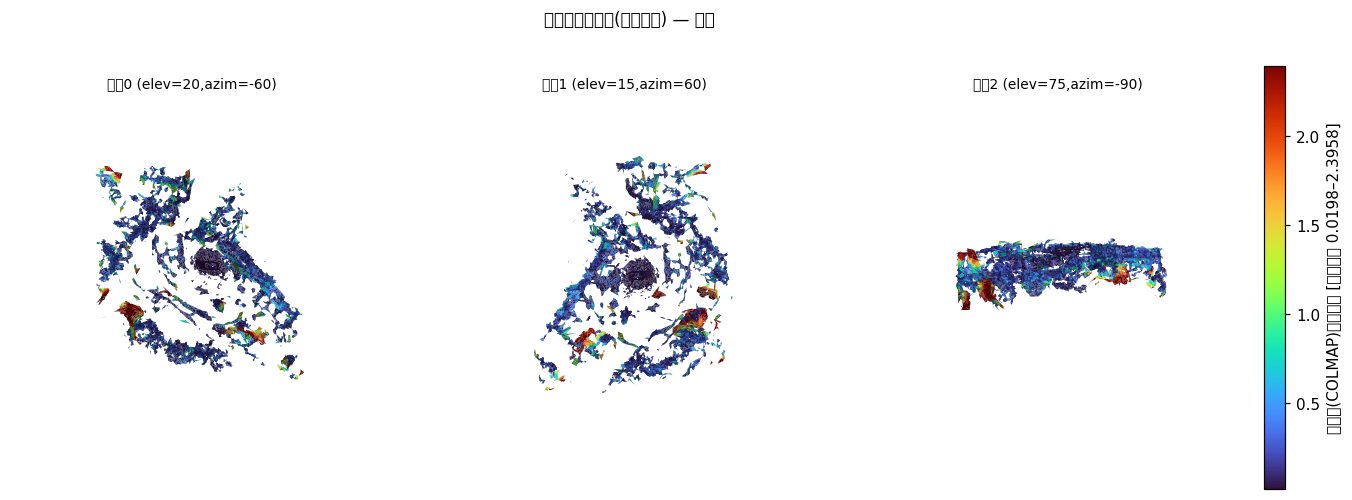
\includegraphics[width=\textwidth]{figures/误差热图_统一色标_基线.png}
    \caption{基线}
  \end{subfigure}
  \hfill
  \begin{subfigure}[b]{0.48\textwidth}
    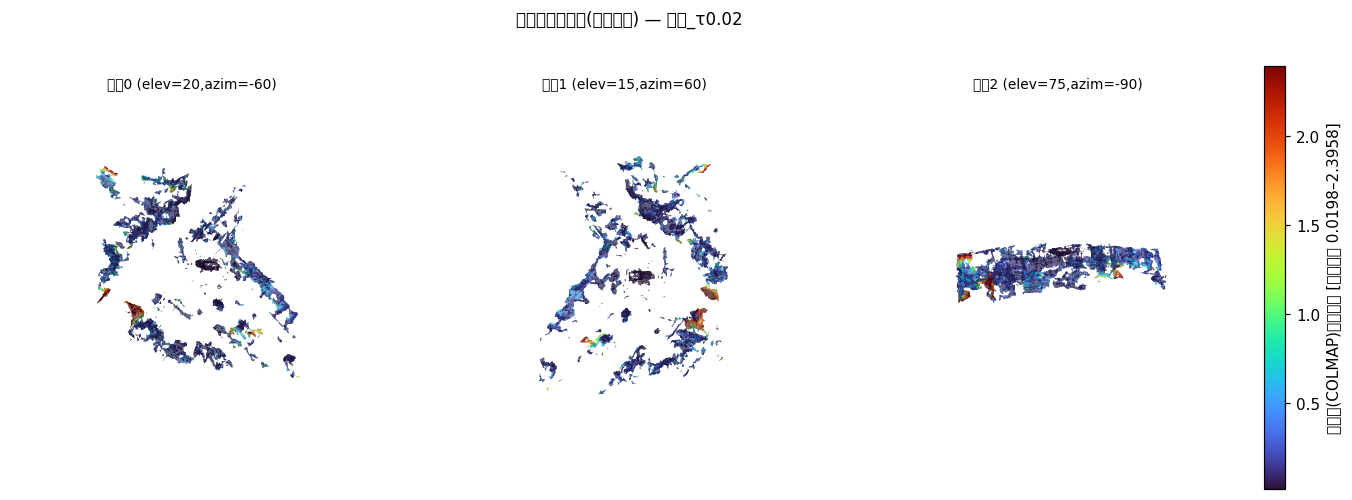
\includegraphics[width=\textwidth]{figures/误差热图_统一色标_改动_τ0.02.png}
    \caption{改动（$\tau{=}0.02$）}
  \end{subfigure}
  \caption{几何误差热图对比（统一色标，单位：场景坐标）。
  剔点后（右），远景区域的大面积高误差区显著减少，
  说明背景壳与漂浮几何被有效剔除；
  但前景主体边缘出现部分孔洞。}
  \label{fig:heatmap-comparison}
\end{figure}

\IfFileExists{figures/对比图_基线_vs_改动.pdf}{%
  \begin{figure}[htbp]
    \centering
    \includegraphics[width=\textwidth]{figures/对比图_基线_vs_改动.pdf}
    \caption{基线与改动（$\tau{=}0.02$）的综合可视化对比：
    网格整体视图、连通分量着色与渲染覆盖掩码。}
    \label{fig:overall-comparison}
  \end{figure}
}{}

% ---------- 基线观察 ----------
\subsubsection{基线观察}
\label{ssec:baseline-obs}

从表~\ref{tab:topo-cov-eff} 与图~\ref{fig:baseline-vis} 可以看出，
基线提取的网格包含~4{,}851 个连通分量，
但最大分量仅占全部面数的约~49.5\%，
说明近半数的三角面分布在数千个漂浮小块中。
这些漂浮几何导致~96{,}544 条边界边与~7{,}970 个孔洞，网格远非水密。
该现象与第~\ref{sssec:motivation}~节分析的单视角自洽但跨视角不一致的
表面采样点直接相关，为后续改动提供了明确的优化方向。

% =====================================================================
\subsection{超参敏感性与失败案例}
\label{ssec:sensitivity}

图~\ref{fig:tau-curve} 展示了剔除率随容差 $\tau$ 的变化趋势。
在固定 $k_{\min}{=}2$、$v_{\max}{=}1$、$M{=}30$ 的条件下，
剔除率随 $\tau$ 严格单调递减：
$\tau{=}0.005$ 时剔除 72.2\%，$\tau{=}0.2$ 时仅剔除 9.0\%。

\begin{figure}[htbp]
  \centering
  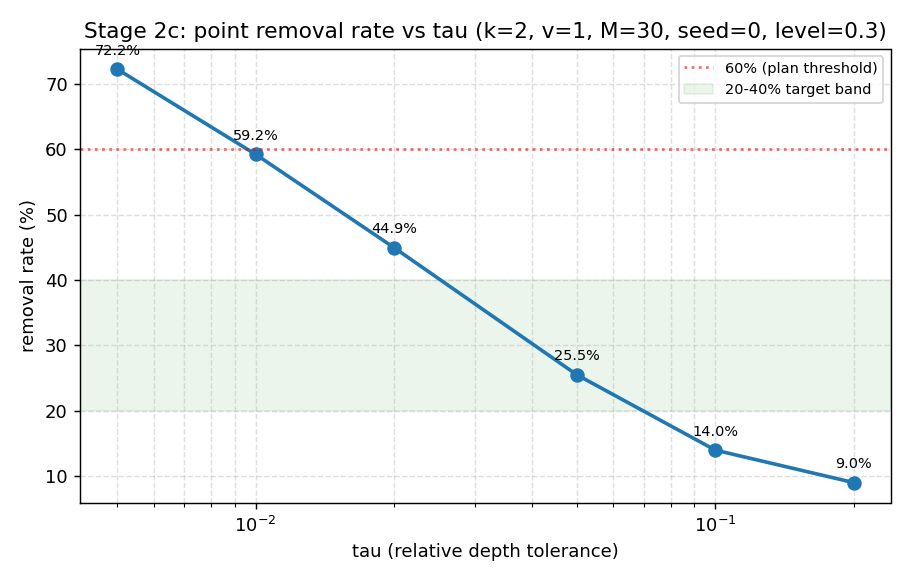
\includegraphics[width=0.65\textwidth]{figures/剔除率_随τ变化.png}
  \caption{剔除率随容差 $\tau$ 的变化（$k_{\min}{=}2$，$v_{\max}{=}1$，$M{=}30$）。
  $\tau$ 越小判据越严格，剔除的点越多。
  本实验选取 $\tau\in\{0.05,\,0.02,\,0.01\}$ 三点做完整提取与评测。}
  \label{fig:tau-curve}
\end{figure}

表~\ref{tab:geo-refA}--\ref{tab:topo-cov-eff} 揭示了 $\tau$ 驱动的一组权衡。
随着 $\tau$ 从 0.05 减小到 0.01：
\begin{itemize}[nosep]
  \item \textbf{改善方向}：连通分量（3{,}279 $\to$ 2{,}261）、
        孔洞（6{,}206 $\to$ 4{,}598）、边界边（68{,}205 $\to$ 44{,}848）
        持续下降；
        Chamfer 距离（参考 B）从 0.0455 降至 0.0361；
        F@1\%（参考 B）从 0.920 升至 0.963。
  \item \textbf{恶化方向}：网格覆盖率从 81.5\% 降至 63.3\%，
        前景漏洞率从 18.0\% 升至 36.3\%；
        Accuracy P90（参考 B）从 0.0239 升至 0.0287（变差 20\%），
        反映部分真实表面被误剔后参考点到最近网格面的距离增大。
\end{itemize}

\paragraph{失败案例：$\tau{=}0.01$。}
$\tau{=}0.01$ 剔除了 59.2\% 的表面点，覆盖率骤降至 63.3\%、
漏洞率飙升至 36.3\%。
虽然 Chamfer 距离仍在改善，但代价已远超收益：
真实表面因深度渲染的微小误差（离散化噪声、遮挡边界处的深度跳变）
被判为不一致而被剔除，形成大面积孔洞。
这一失败案例表明，$\tau$ 不应低于深度渲染本身的噪声水平。

\paragraph{推荐设置。}
$\tau{=}0.05$ 仅剔除 25.5\%，拓扑改善温和、覆盖损失可控（81.5\%）；
$\tau{=}0.02$ 剔除 44.9\%，几何收益更显著但覆盖降至 71.0\%。
二者的选择取决于下游任务对覆盖完整性与几何干净度的相对权重。

% =====================================================================
\subsection{分析}
\label{ssec:analysis}

\paragraph{改动带来了什么。}
多视角深度一致性剔点在所有 $\tau$ 设置下均显著降低了 Chamfer 距离
（参考 B：基线 0.0531 $\to$ $\tau{=}0.02$ 时 0.0390，降幅约 27\%）、
连通分量数（4{,}851 $\to$ 2{,}690，降幅 45\%）与孔洞数
（7{,}970 $\to$ 5{,}480，降幅 31\%）。
Completeness 均值大幅改善（参考 A：0.0495 $\to$ 0.0286，降幅 42\%），
表明漂浮于远离参考面的虚假网格面已被有效消除。
F-score 在所有阈值下均单调上升
（F@1\% 参考 B：0.888 $\to$ 0.949），
进一步证实剔点在保持召回率的同时大幅提升了精确率。
在 $\tau{=}0.05$ 时，最大分量面数占比从 49.5\% 升至 58.1\%，
意味着网格几何更集中于场景主体。

\paragraph{改动没有带来什么。}
渲染质量完全不变（PSNR 24.32\,dB、SSIM 0.848），
这是设计上的必然结果：改动仅作用于 Mesh 提取阶段，
Coarse SuGaR 模型未经重训练，其高斯分布不受影响。
此外，网格在任何 $\tau$ 下均未达到水密状态——
Poisson 重建本身产生开放边界，仅靠剔点无法弥补。

\paragraph{计算代价。}
过滤器本身的额外开销极小：渲染 30 个参考深度图约 0.3\,s，
投票判断约 0.2\,s，合计约 0.5\,s。
由于剔点后进入 Poisson 重建的点数减少，
总提取墙钟反而缩短——$\tau{=}0.02$ 时从 5.98\,min 降至 4.30\,min（快 28\%）。
峰值显存在 $\tau{=}0.02$ 下为 8{,}274\,MiB，低于基线的 10{,}098\,MiB。
因此，该改动在计算成本上几乎"免费"。

\paragraph{覆盖率下降是主要代价。}
网格覆盖率从基线的 92.9\% 降至 $\tau{=}0.02$ 时的 71.0\%，
前景漏洞率从 6.7\% 升至 28.6\%，
这是本改动的最大不足。
Accuracy P90（参考 B）从 0.0200 升至 0.0258（变差 29\%），
说明剔点误伤了部分真实表面，
使一些参考点失去了近邻网格面。

\paragraph{假设对照。}
实验结果逐条验证了三项预注册假设：

\begin{enumerate}[nosep,label=\textbf{H\arabic*}:]
  \item \textbf{几何改善}——
        连通分量数、Chamfer 距离、Completeness 均值三项均随剔点
        单调改善（\textbf{支持}）。
  \item \textbf{过剔损害覆盖}——
        $\tau$ 越小，覆盖率越低、漏洞率越高、Accuracy P90 越差；
        $\tau{=}0.01$ 构成典型的过度剔除案例（\textbf{支持}）。
  \item \textbf{渲染不变}——
        所有组别共享同一 Coarse 模型，PSNR / SSIM / LPIPS 恒等
        （\textbf{支持}）。
\end{enumerate}

% sec4_conclusion.tex — 第4节 总结
\section{总结}

本报告在 truck 场景上完成了 3DGS $\to$ Coarse SuGaR $\to$ Mesh 提取的基线复现，
并提出了 Poisson 重建前的多视角深度一致性剔点改动。
$\tau{=}0.02$ 时 Chamfer 距离（参考 B）从 0.0531 降至 0.0390，
连通分量数从 4{,}851 降至 2{,}690，提取墙钟缩短约 28\%；
代价是覆盖率从 92.9\% 降至 71.0\%。
三条预注册假设（H1 几何改善、H2 过剔损覆盖、H3 渲染不变）均获实验支持。

\paragraph{局限性。}
(1) 缺乏真值网格，几何评测仅依赖 3DGS 高斯中心与 COLMAP 稀疏点两个代理参考；
(2) 仅在 truck 单场景验证，结论向室内或大规模场景的推广性未知；
(3) 改动仅作用于提取阶段，未重训 Coarse SuGaR，无法评估端到端收益。

\paragraph{下一步。}
(1) 将一致性判据前移至 Coarse 训练阶段做正则项，从源头抑制虚假密度峰；
(2) 在投影误差项中加大跨视角不一致点的惩罚权重，替代后处理式剔点；
(3) 扩展至更多场景与 refined SuGaR 阶段，评估端到端效果。


% ---- 参考文献 ----
\bibliographystyle{plainnat}
\bibliography{refs}

% ---- 附录 ----
% appendix.tex — 附录
\appendix
\section{附录}

\subsection{多视角深度一致性剔点的超参数}

\begin{table}[H]
\centering
\caption{多视角深度一致性剔点的超参数}
\label{tab:mv-hyperparams}
\begin{tabular}{llp{7cm}}
\toprule
\textbf{符号} & \textbf{默认值} & \textbf{含义} \\
\midrule
$\tau$     & 0.02  & 相对深度容差，$|z_p - z_{\mathrm{map}}|/z_{\mathrm{map}} < \tau$ 即判一致 \\
$k_{\min}$ & 2     & 保留所需的最少一致票数 \\
$v_{\max}$ & 1     & 允许的最大空域冲突票数 \\
$M$        & 30    & 参考相机抽样数（均匀抽取，\texttt{seed}=0） \\
\bottomrule
\end{tabular}
\end{table}

\subsection{算法伪代码}

\begin{algorithm}[H]
\SetKwInOut{Input}{输入}
\SetKwInOut{Output}{输出}
\SetKwFunction{Render}{RenderDepth}
\SetKwFunction{Project}{Project}
\SetKwFunction{GetDepth}{GetMapDepth}
\caption{多视角深度一致性剔点（Multi-view Depth Consistency Filter）}
\label{alg:mv-filter}
\Input{表面点集 $\mathcal{P}$，SuGaR 模型，训练相机 $\mathcal{C}$，\\
       超参 $\tau, k_{\min}, v_{\max}, M$}
\Output{过滤后的点集 $\mathcal{P}'$}
$\mathcal{C}_M \leftarrow$ 从 $\mathcal{C}$ 均匀抽样 $M$ 个相机（\texttt{seed}=0）\;
\ForEach{$c_j \in \mathcal{C}_M$}{
  $D_j \leftarrow$ \Render{SuGaR, $c_j$} \tcp*{缓存渲染深度图}
}
\ForEach{$p_i \in \mathcal{P}$}{
  $n_{\mathrm{con}} \leftarrow 0$;\quad $n_{\mathrm{cfl}} \leftarrow 0$\;
  \ForEach{$c_j \in \mathcal{C}_M$}{
    $(u, v, z_p) \leftarrow$ \Project{$p_i$, $c_j$}\;
    \If{$(u, v)$ 在视锥内}{
      $z_{\mathrm{map}} \leftarrow D_j(u, v)$\;
      \uIf{$|z_p - z_{\mathrm{map}}| < \tau \cdot z_{\mathrm{map}}$}{
        $n_{\mathrm{con}} \leftarrow n_{\mathrm{con}} + 1$\;
      }
      \uElseIf{$z_p < z_{\mathrm{map}} - \tau \cdot z_{\mathrm{map}}$}{
        $n_{\mathrm{cfl}} \leftarrow n_{\mathrm{cfl}} + 1$\;
      }
    }
  }
  \If{$n_{\mathrm{con}} \geq k_{\min}$ \textbf{且} $n_{\mathrm{cfl}} \leq v_{\max}$}{
    将 $p_i$ 加入 $\mathcal{P}'$\;
  }
}
\Return $\mathcal{P}'$\;
\end{algorithm}


\end{document}
